\section{Datenbus}
Eines der Hauptbestandteile des modularen Eingabesystems ist das Entwerfen und Umsetzen eines leistungsfähigen und flexiblen Datenbusses. Dieser Datenbus dient als Kommunikationsschnittstelle zwischen den verschiedenen Modulen, wie dem Keypad-Modul und dem Audiomodul und ermöglicht dadurch die Datenübertragung zum Hauptmodul. Skalierbarkeit, Zuverlässigkeit und Geschwindigkeit sind die Hauptkriterien des Datenbusses. Ziel ist es, eine einfache Erweiterbarkeit durch Hinzufügen oder Entfernen von Modulen zu ermöglichen, ohne dabei grundlegende Kommunikationsmechanismen zu beeinträchtigen.

\subsection{Aufbau des Datenbusses}
Der Bus ist nach folgendem Schema aufgebaut:
\begin{itemize}
	\item \textbf{Start of Frame (SOF):} 2 Bit zum Synchronisieren der Frequenzen; durch einen HIGH-Value wird der Beginn des SOF bekanntgegeben und durch das darauf folgende LOW-Value können die Teilnehmer sich auf die Übertragungsgeschwindigkeit synchronisieren.
	\item \textbf{Sendeadresse:} 3 Bit zum Senden der Adresse; Die Adresse 0x00 ist für neue Teilnehmer reserviert, über diese Adresse findet die Adressvergabe statt. Die Adresse 0x01 ist fest an das Hauptmodul vergeben, alle Teilnehmer wissen das auf dieser Adresse das Hauptmodul liegt. Die Adressen 0x02 bis 0x07 stehen für Teilnehmer zur Verfügung. 3 Bit sind vollkommen ausreichend, da das System als Desktop Erweiterung geplant ist und mehr als 6 Module nicht vorgesehen ist. Sollten in Zukunft mehr Teilnehmer erforderlich sein, lässt sich das im Code leicht anpassen.
	\item \textbf{Content of Frame (COF):} 3 Bit für Datenlänge in Byte; das COF enthält die Länge der übertragenden Daten in Byte. Dies dient dazu, dass die Länge der zu übertragenden Daten dynamisch sein kann (bis zu 7 Byte). Zusätzlich können Teilnehmer, welche nicht angesprochen werden, festlegen, wie lange der Bus belegt ist, bevor diese versuchen sollten zu senden.
	\item \textbf{Daten}: 0-7 Byte
	\item \textbf{Fehlererkennung (CRC):} 15 Bit; Mithilfe eines 16-Bit Generatorpolynom lassen sich bis zu 15-Bit Fehler erkennen. Eine fehlerhafte Nachricht soll ignoriert werden. 
	\item \textbf{End of Frame (EOF):} 4 Bit Signalende; Vier aufeinanderfolgende LOW-Values geben das Ende der Nachricht an. Ein Teilnehmer, der Senden möchte, wartet bis er 4 aufeinanderfolgende LOW-Value empfangen hat, bevor dieser Sendet.
\end{itemize}

In Abbildung \ref{Datenbus} ist eine grafische Darstellung des Busaufbau zu sehen.
\begin{figure}[H]
	\centering    
	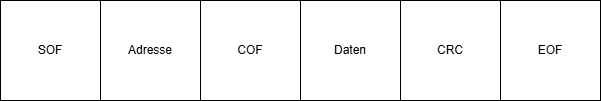
\includegraphics[width=1\textwidth]{Bilder/datenbus.png}
	\caption{Aufbau des Datenbusses}
	\label{Datenbus}
\end{figure}

\subsection{Technische Eigenschaften}
Zu dem jetzigen Zeitpunkt kann der selbst erstellte Bus Informationen mit einer Geschwindigkeit von $250\frac{\mathrm{Byte}}{\mathrm{s}}$ übertragen. Dabei kann eine maximale Teilnehmeranzahl (Eingabemodule) von sieben erreicht werden. Dies liegt hauptsächlich an den Adressierungsbits des Busses und könnte beliebig erweitert werden. Die Datensignale haben einen Pegel von 0\,\si{V} bis 3,3\,\si{V}

\begin{figure}[H]
    \centering    
    \fbox{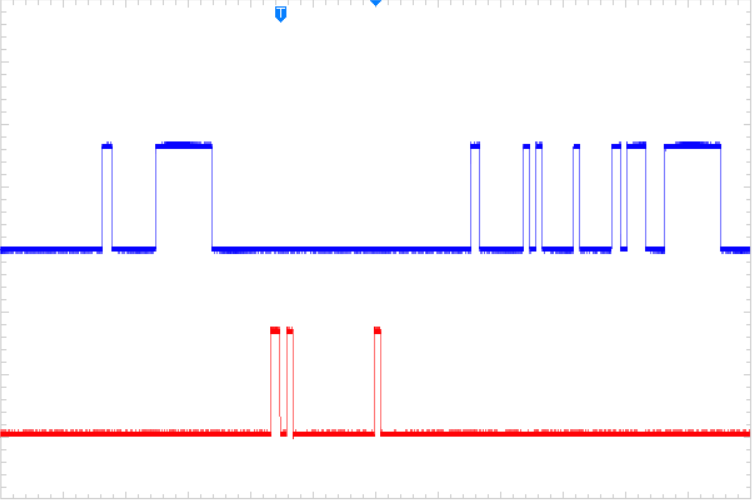
\includegraphics[width=0.8\textwidth]{Bilder/Datenaustausch.png}}
    \caption{Kommunikation zwischen zwei ESP32 über unseren Datenbus.}
    \label{zeitplan}
\end{figure}

\begin{figure}[H]
    \centering    
    \fbox{\includegraphics[width=0.8\textwidth]{Bilder/Beispiel_Datenübertragung.png}}
    \caption{Beispiel differenzielle Datenübertragung}
    \label{beispielDatenübertragung}
\end{figure}

\subsubsection{CRC Fehlererkennung}
Zur Erkennung von Bitfehlern wird das 16-Bit Generatorpolynom in Abbildung \ref{CRC-Polynom} genutzt. 
\begin{figure}[H]
	\centering    
	\fbox{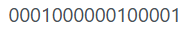
\includegraphics[width=0.5\textwidth]{Bilder/CRC.png}}
	\caption{CRC-16-Bit Generatorpolynom (0x1021)}
	\label{CRC-Polynom}
\end{figure}


\begin{lstlisting}[caption={CRC-Encoder Funktion. Noch nicht implementiert, dies ist lediglich ein Ansatz der noch im Programm einzubinden ist.}, label={lst:crcEncode}]
void crcEncode(){
 uint64_t remainder;
		
 for(int i = 0; i < 8; i++){
  // merge the message into a single variable
  encodedMessage = (encodedMessage << 8) 
   | (uint8_t)global_message[i]; 
 }
 // append as many zeroes as the degree of the polynomial - 1
 remainder = encodedMessage << 15; 
 // divide the message with the generator polynomial
 for(int i = 15; i > 0; i--){
  // check for leading 0 -> no XOR while a leading 0
  if((remainder << i+1) != 0){
   remainder = remainder ^ (generator_polynomial << i);
  }
 }
 // append remainder to message
 // should only append the remainder after the division
 encodedMessage = (encodedMessage << 15) | remainder   
}
	
\end{lstlisting}

\begin{lstlisting}[caption={CRC-Decoder Funktion. Noch nicht implementiert, dies ist lediglich ein Ansatz der noch im Programm einzubinden ist.}, label={lst:crcDencode}]
void crcDecode(){
 uint64_t remainder;
 uint64_t message;           // message received
	
 for(int i = 15; i >= 0; i--){
  // check for leading 0 -> no XOR while a leading 0
  if((remainder << i+1) != 0){
   remainder = remainder ^ (generator_polynomial << i);
  }
 }
		
 for(int i = 0; i < 17; i++){
  if((remainder & (0x01 << i)) == 0x01){
   // ERROR in the message, ignore this message
   break;
  } 
 }
}
	
\end{lstlisting}


Mit diesem Generatorpolynom lassen sich folgende Fehler erkennen:
\begin{itemize}
	\item \textbf{Single-Bit Errors:} alle Fehler
	
	\item \textbf{Double-Bit Errors:} alle Fehler, solange die Distanz zwischen den Fehlern kleiner als 16 Bit ist
	
	\item \textbf{Burst Errors:} bis zu 16 Bit 
\end{itemize}

\subsubsection{Bitstuffing}
Da jeder Teilnehmer auf den Bus hört und auf das EOF wartet bevor eine neue Nachricht gesendet wird, haben wir ein 3-Bit Bitstuffing eingebaut. Entsprechend wird nach dem dritten gleichen Bit ein invertiertes Bit eingefügt.

\begin{figure}[H]
	\centering    
	\fbox{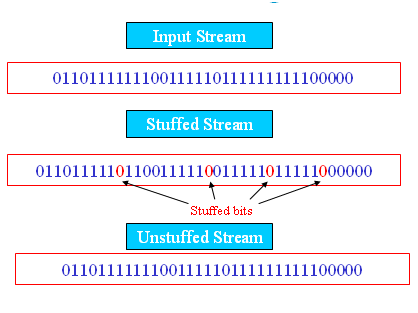
\includegraphics[width=0.8\textwidth]{Bilder/bitstuffing.png}}
	\caption{Darstellung von Bitstuffing an einem Beispiel. In diesem Beispiel handelt es sich um 5-Bit Bitstuffing. [https://prayasnotty.wordpress.com/wp-content/uploads/2010/11/bit12.png, 17.01.2025]}
	\label{bitstuffing}
\end{figure}